\section{Durchführung}
\label{sec:Durchführung}

\subsection{Zeitkonstante eines RC-Kreises}

\begin{figure}
    \centering
    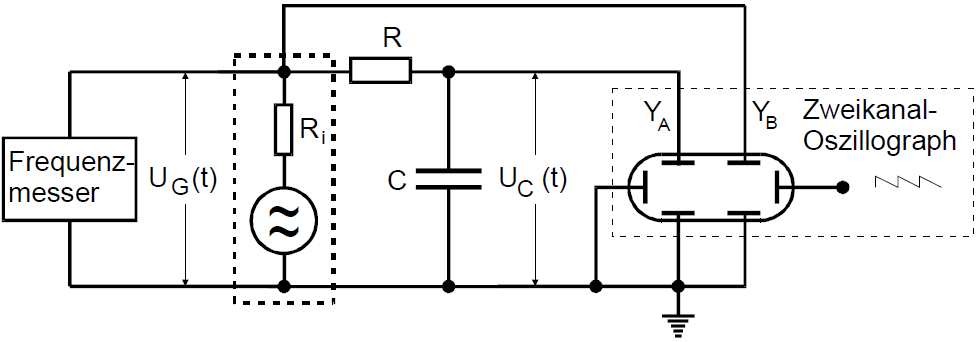
\includegraphics[height=6cm]{data/bild_4}
    \caption{Aufbau zur Messung der Kondensatorspannungsamplitude und der Phasenverschiebung}
    \label{fig:bild_4}
\end{figure}

\begin{figure}
    \centering
    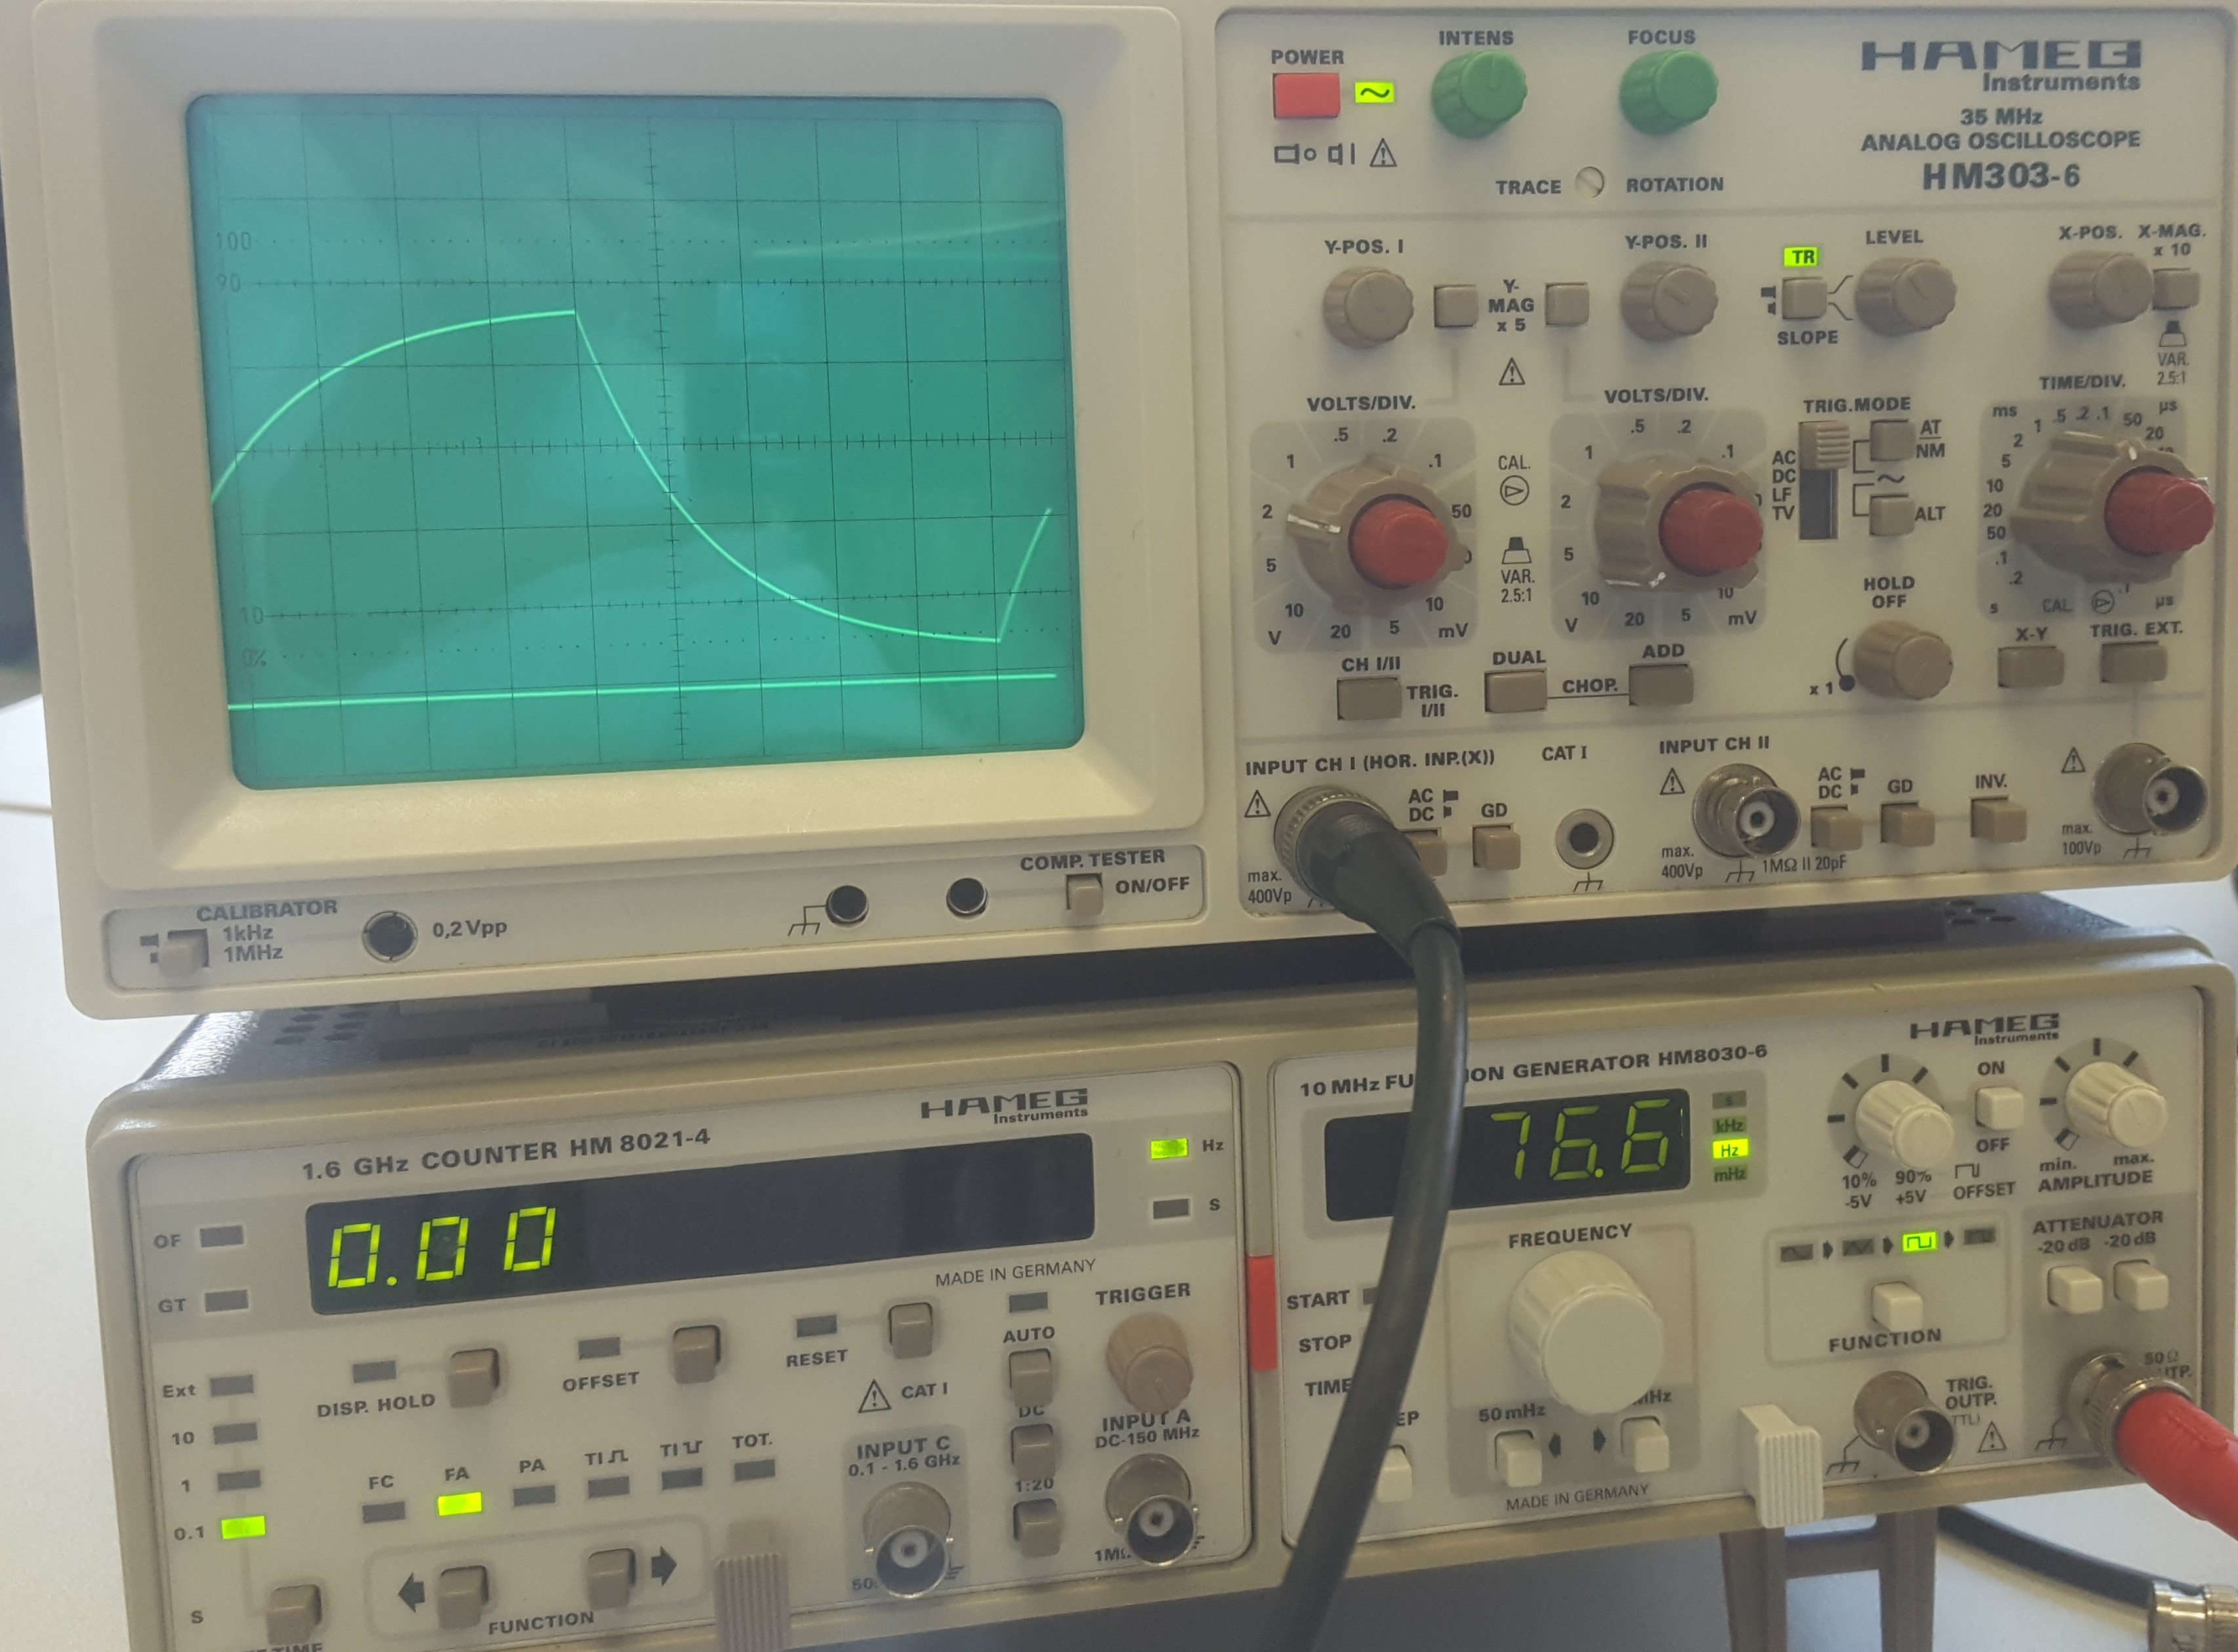
\includegraphics[height=6cm]{data/a_zeitkonstante}
    \caption{Messung zur Bestimmung der Zeitkonstante}
    \label{fig:a_zeit}
\end{figure}

Es wird, wie in Abb. \ref{fig:bild_4} der RC-Kreis an eine Rechteckspannung angeschlossen und die Kondensatorspannung 
anhand eines Oszilloskops abgelesen. Dafür wird vorerst der Spannungsnullpunkt ermittelt , indem die Frequenz der 
Speisespannung ausreichend gering eingestellt wird, dass es beim Entladevorgang zu einem völligen Entladen des Kondensators kommt. 
Danach kann wieder eine höhere Frequenz genutzt werden, die so gewählt wird, dass jeweils das Anfangsstadium eines Auf- oder 
Entladevorgangs gut so erkennen ist. In diesem bieten sich Messungen am besten an, da die Änderungrate der Spannung in diesem 
Bereich am größten ist.
Es wird innerhalb eines Auf- oder Entladevorgangs die Kondensatorspannung an mehreren Zeitpunkten abgelesen, wodurch der zeitliche 
Verlauf und somit die Zeitkonstante von $U_C (t)$ ermittelt werden kann.

\subsection{Amplitude und Phasenverschiebung}
Bei einer am RC-Kreis anliegenden Sinusspannung $U(t)$ wird die frequenzabhängige Amplitude der Kondensatorspannung untersucht.
Mit dem selben Aufbau lässt sich außerdem die ebenfalls frequenzabhängige
Phasenverschiebung von Kondensatorspannung zu Speisespannung ermitteln.
Dabei wird auf einem Zweikanal-Oszilloskop die Speisespannung $U(t)$ und simultan die Kondensatorspannung $U_C (t)$ abgebildet.
Die Frequenz wird dabei von $100\si{\hertz}$ bis $1000\si{\hertz}$ in hunderter Schritten variiert. Es wird jeweils die 
Kondensatorspannungsamplitude und die Phasenverschiebung abgelesen. Wichtig ist dabei, darauf zu achten, dass beide Spannungsverläufe
zur $x$-Achse symmetrisch sind. 

\subsection{RC-Kreis als Integrator}
Der Aufbau bleibt für diesen Versuch unverändert.
Bei einer Frequenz von $20\si{\kilo\hertz}$ wird als Speisespannung nacheinander eine Sinus-, Rechteck- und Dreiecksspannung
verwendet. Neben dieser wird auf dem Oszilloskop auch die Kondensatorspannung angezeigt. Es wird jeweils ein Foto der beiden 
Spannungsverläufe gemacht, wie sie in Abb \ref{fig:sinus}, \ref{fig:dreieck} und \ref{fig:rechteck} zu sehen sind. 

\begin{figure}
    \centering
    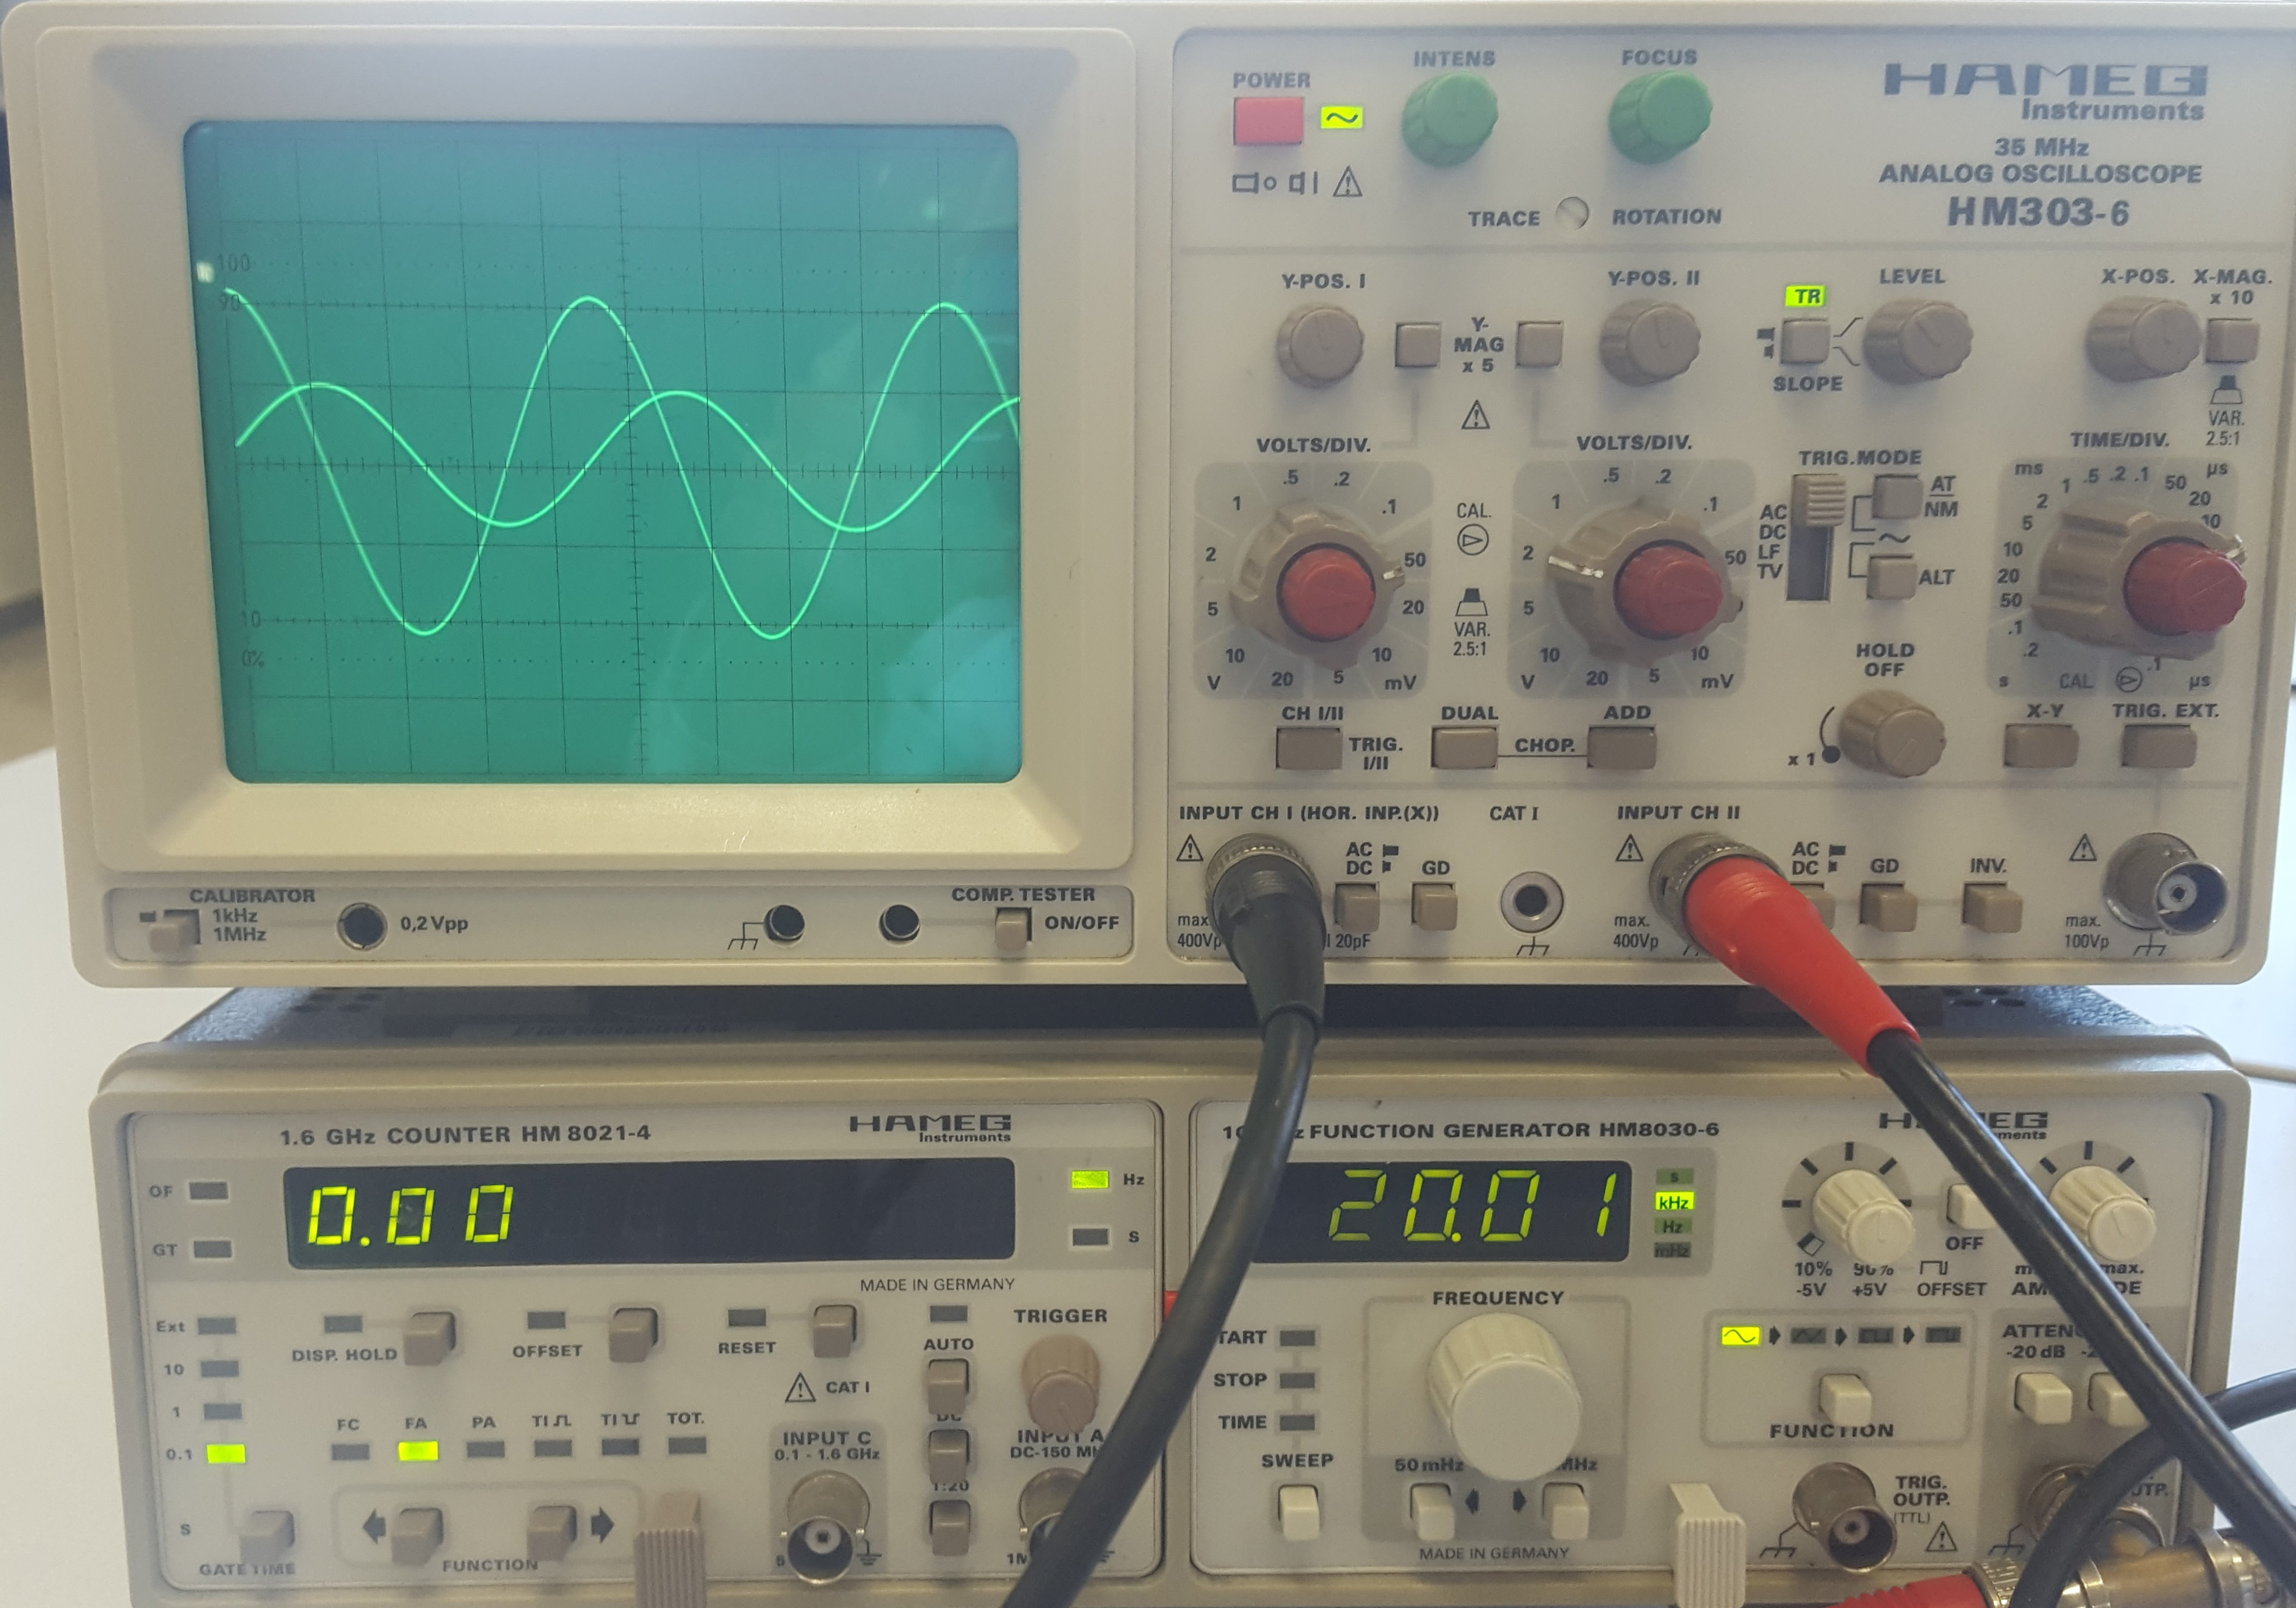
\includegraphics[height=6cm]{data/d_sinus}
    \caption{Sinusspannung}
    \label{fig:sinus}
\end{figure}

\begin{figure}
    \centering
    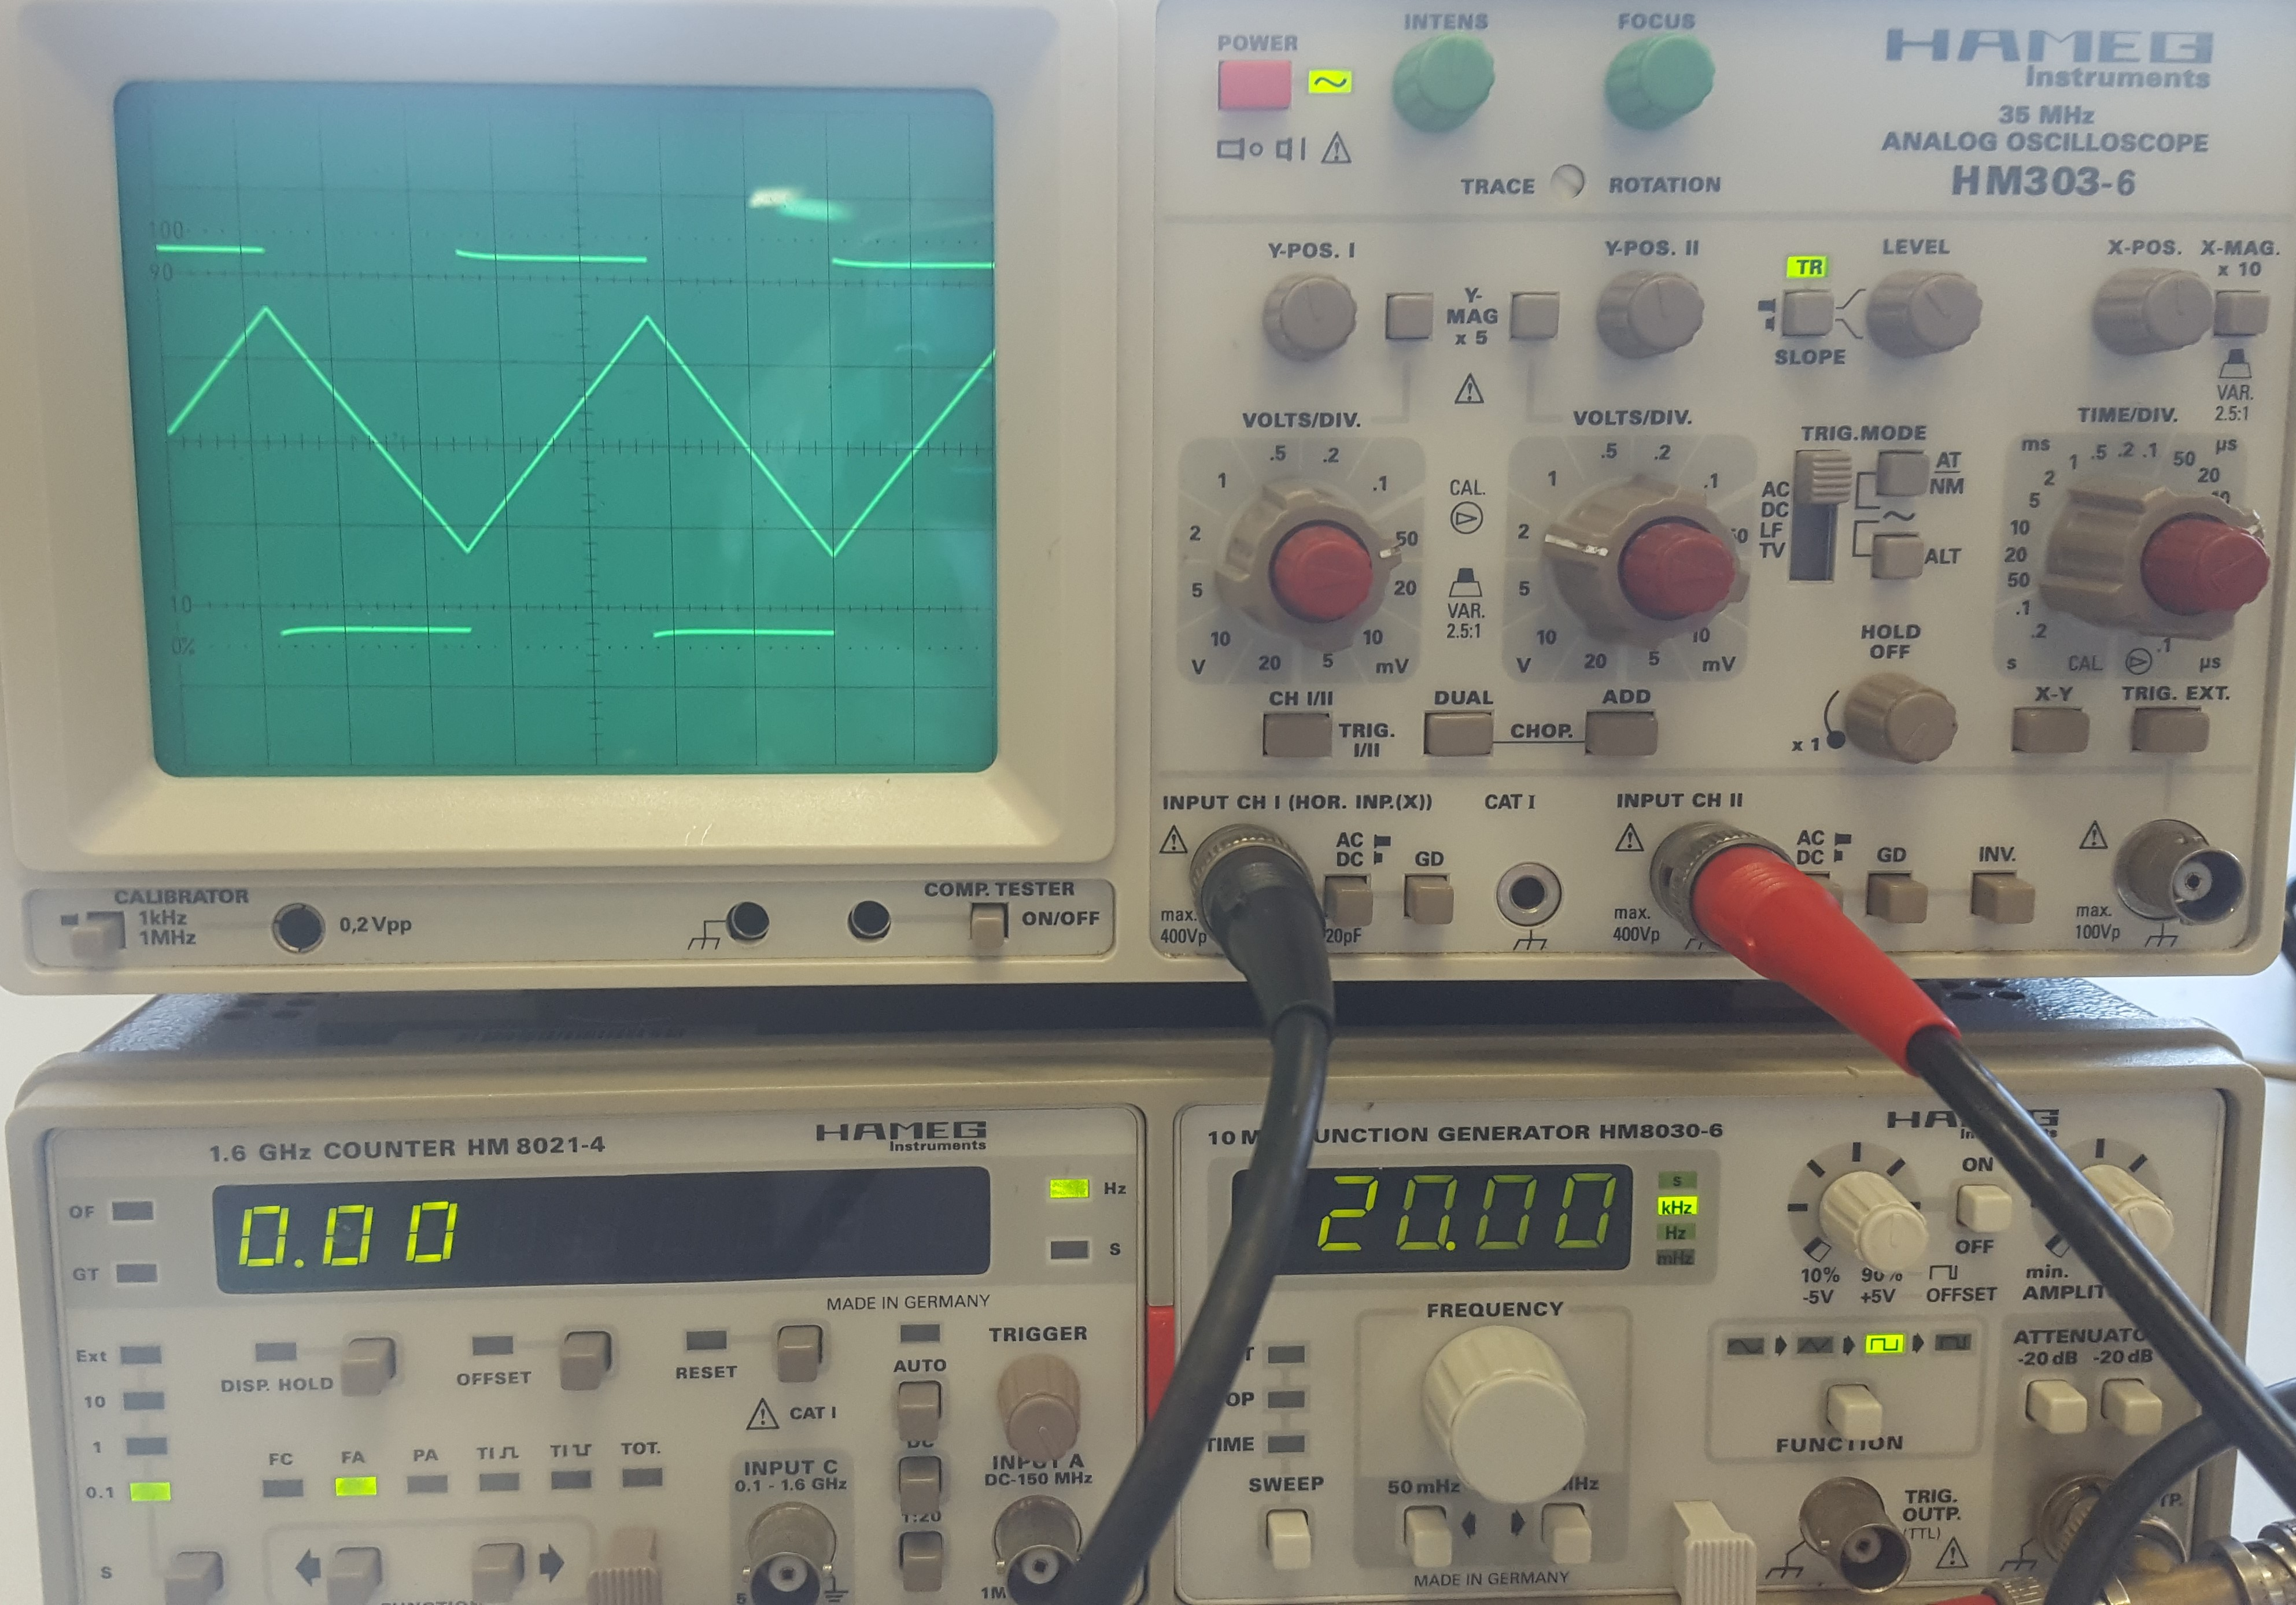
\includegraphics[height=6cm]{data/d_rechteck}
    \caption{Rechteckspannung}
    \label{fig:rechteck}
\end{figure}

\begin{figure}
    \centering
    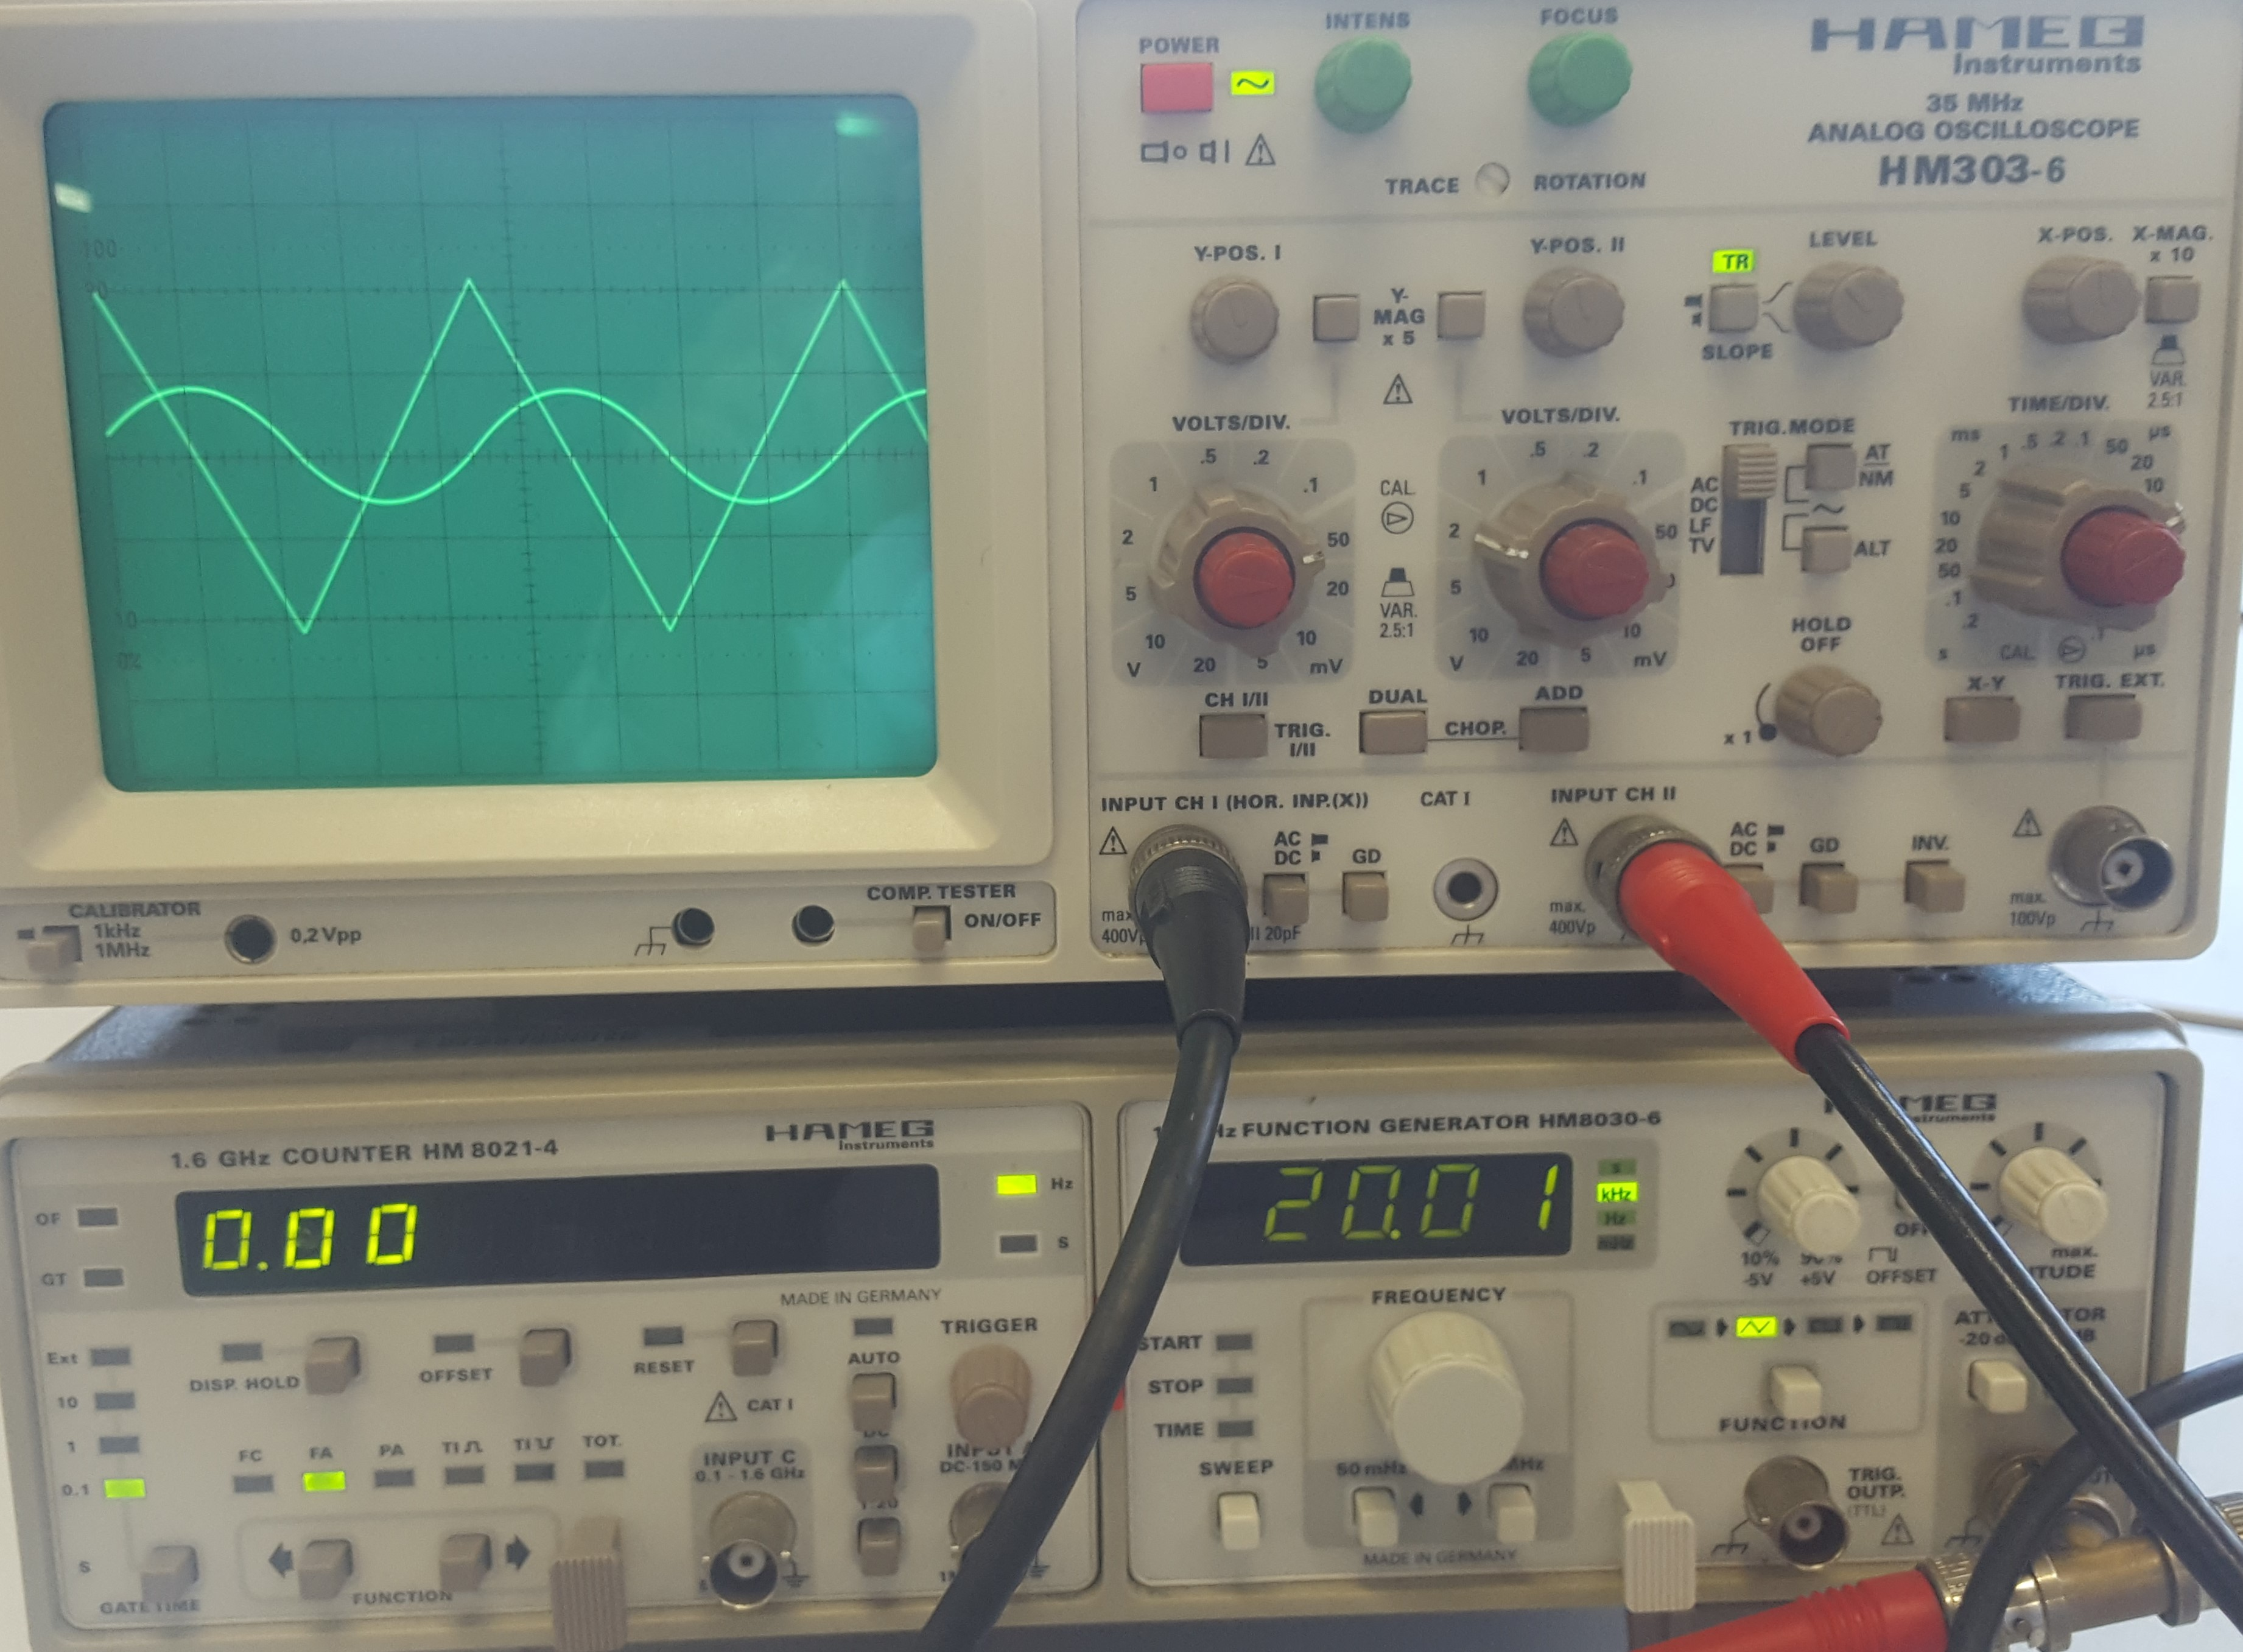
\includegraphics[height=6cm]{data/d_dreieck}
    \caption{Dreiecksspannung}
    \label{fig:dreieck}
\end{figure}

%Was wurde gemessen bzw. welche Größen wurden variiert?